\section{\Glsfmtlong{nmt}}

La deuxième partie de notre système (et celle qui réalise sa fonction principale) est le modèle de traduction.
Ce modèle corrige la parole aphasique pour la rendre plus compréhensible.
La procédure de sa création est décrite dans la Figure~\ref{fig.nmt-archi}.
Dans cette section, nous allons détailler les étapes de sa construction.

\begin{figure}[hbt]
    \begin{center}
        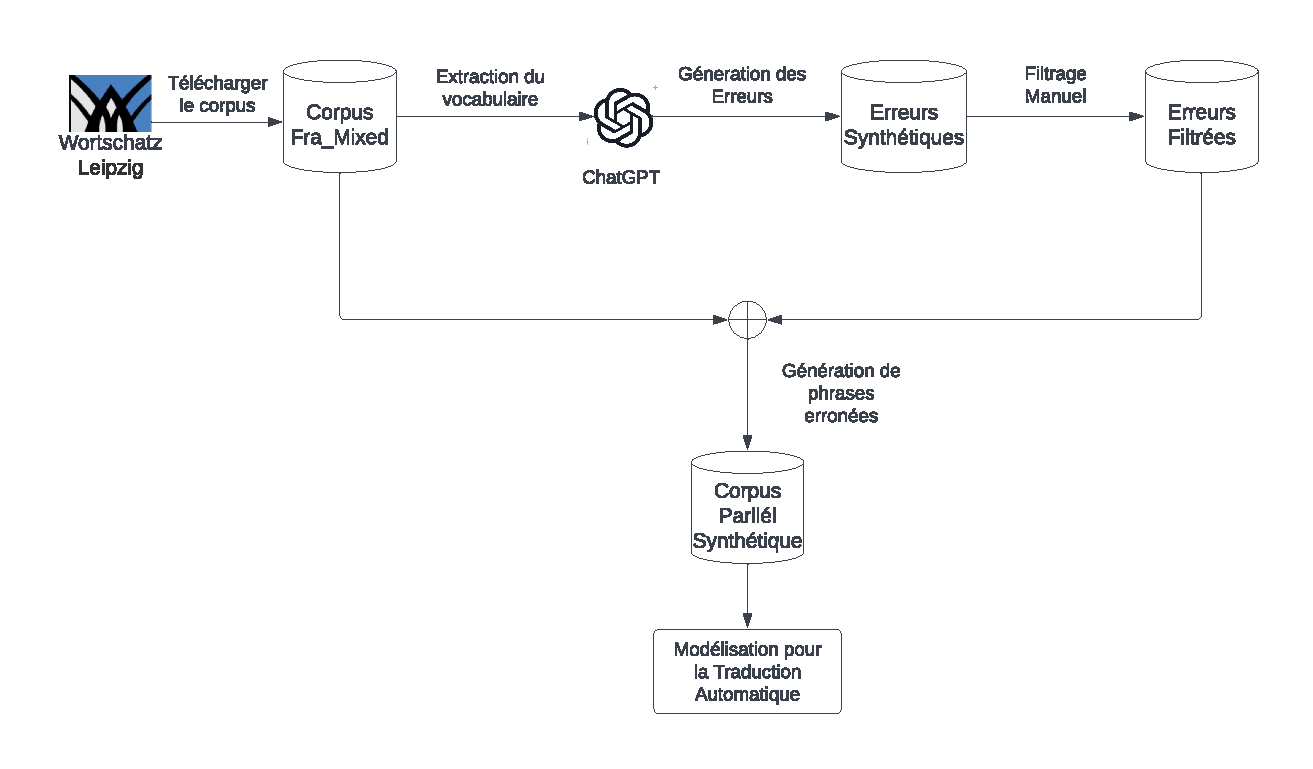
\includegraphics[width=\textwidth]{assets/pdf/NMT.pdf}
    \end{center}
    \caption{Déroulement de la partie \glsfmtshort{nmt}.}
    \label{fig.nmt-archi}
\end{figure}


\subimport{}{corpus}
\subimport{}{model}
\subimport{}{train}
\subimport{}{eval}